\documentclass[11pt]{jsarticle}
\usepackage{amsmath,amssymb} % 数式を使うため
\usepackage{mathdots} % 数式内の右肩上がり3点 \iddots
\usepackage{bm} % ベクトルの太字 \bm{}
\usepackage{ascmac} % 枠で囲む環境 itembox, screen, boxnote, shadebox
\usepackage{booktabs} % 欧米風のテーブル環境 \tabular の中で \toprule,\midrule, \bottmrule
\usepackage{multirow} % テーブルの複数行に渡る項目 \multirow{行数}{*}{内容}
\usepackage[dvipdfmx,bookmarks=true,bookmarksnumbered=true]{hyperref} % PDF 文書内に URL へのリンクを貼る \url{アドレス}
\usepackage{pxjahyper} % 日本語のしおりを付けるため。hyperref と対で使用
\hypersetup{colorlinks=true,linkcolor=blue, citecolor=blue, urlcolor=blue} % リンクを下線からカラーリンクに変更。hyperref と対で使用
\usepackage{listings, jlisting} % ソースコードを書くため \begin{lslisting}\end{lslistiing}
\def\lstlistingname{ソースコード}
\lstset{%
	tabsize = 3, % タプインデントの大きさ
	basicstyle = \footnotesize, % 基本の文字スタイル
	keywordstyle = \bfseries\color{blue}, % キーワード
	stringstyle = \color{red}, % 文字列
	showstringspaces=false,
	commentstyle = \color[rgb]{0,0.5,0}, % コメント
	framesep = 10pt, % 
	xleftmargin = 20pt, % 左インデント
	xrightmargin = 20pt, % 右インデント
}
\lstdefinestyle{MATLABStyle}{%
	language = Matlab,
	frame=single, % フレームの書式
	backgroundcolor = {\color[gray]{0.96}}, % 背景色を灰色
	numbers = {left}, % 行番号の位置
	numberstyle = {\footnotesize}, % 行番号のスタイル
	numbersep = {2zw}, % コードから行番号までの距離
	morekeywords = {cout, cin, end}
}
\usepackage[hiresbb,dvipdfmx]{graphicx} % PDF, PNG, JPEG, EPS の画像を扱うため
\usepackage{wrapfig} % 図などを文章が回り込むように \begin{wrapfigure} \begin{wraptable}
\usepackage{makeidx} % 索引を作るため \makeindex と対に
\makeindex % 索引を作る:索引をおきたい場所に \printindex を置く

\newtheorem{theorem}{定理}[section]	% 定理環境の定義
\newtheorem{defi}{定義} 		% 定義環境の定義
\newtheorem{coro}{系}		% 系環境の定義
\newtheorem{lemm}{補題} 		% 補題環境の定義

\newcommand{\ten}[1]{{{}^t #1}} % 行列ベクトルの転置 tA を書くため \ten{A}
\renewcommand{\vec}[1]{\bm{#1}} % \bm{x} の代わりに \vec{x}

\newcommand{\inpro}[2]{{\vec{#1}^t\vec{#2}}}

\newenvironment{pocketList}{
   \begin{center}
   \begin{tabular}{ccc} \toprule
   名前 & 分類 & 特性 \\ \midrule
}{
   \\ \bottomrule
   \end{tabular}
   \end{center}
}

\setcounter{tocdepth}{3} % subsubsection まで目次に載せる=3, subsection=2, section=1

%%%%%%%%%%%%%%%%%%%%%%%%%%%%%%%%%%%%%%%%%%%%%%%%%%%%%%%%%%%%%%%%%%
\begin{document}


%1.実験に見合ったタイトル, 学籍番号, 氏名, 日付などを記した表紙をつける
\title{数値解析学}
\author{Sumire}
\date{2022年 8月1日}
\maketitle

%表紙にメモ(概要)
\begin{abstract}
\centerline{Euler法を用いて様々な常微分方程式の数値解, 解の様子, }
\centerline{Euler法の誤差と時間刻み幅 $h = T / N$, 最大計算時間 $T$ の関係について述べる}
\end{abstract}

\clearpage
%目次
\tableofcontents

\clearpage
%表目次
\listoftables
%図目次
\listoffigures

\clearpage



%%%%%%%%%%%%%%%%%%%%%%%%%%%%%%%%%%%%%%%%%%%%%%%%%%%%%%%%%%%%%%%%%%
%2.実験目的(実験を行う動機や背景となった問題点などを述べて目的を明確にする)
\section{実験目的}
微分方程式論について, すでに学習していたため最も興味を持った. また, 常微分方程式(未知数とその導関数含み, 独立変数が1つの方程式)について学び, 微分方程式が物理学・工学といった学問だけでなく, 身近に起きている現象を予測し, 説明することができると知った. \par
ただ計算するだけでなく, 背景を理解し, 応用性を持った学習をしたいと思い, 常微分方程式についてこの課題で扱うことにした. 



%%%%%%%%%%%%%%%%%%%%%%%%%%%%%%%%%%%%%%%%%%%%%%%%%%%%%%%%%%%%%%%%%%

\section{問題設定}
Euler法を用いて常微分方程式の数値解, 解の様子, Euler法の誤差と時間刻み幅 $h = T / N$, 最大計算時間 $T$ の関係を考える。\\
今回は, 以下の2つを扱う\\
\ \ \ \ \ \ \ \ (a)連立線形常微分方程式\\
\ \ \ \ \ \ \ \ (d)(拡散項なしの)藤田方程式\\
\\
※ただし、方程式 $\frac{dx}{dt} = f(t, x(t))$ の真の解が分からない場合, 十分大きな時間ステップ $N'$ をとって(例えば $N' = 20000$), 解$x^{(N')}$ を求める. $x^{(N')}$ は真の解と十分近いので, 真の解とみなす. さらに, $N = 100, 200, ..., 1000$ に対して, $x_{N}$ を計算し, $|x^{(N)} - x^{(N')}|$ を誤差とする. 



\clearpage
%%%%%%%%%%%%%%%%%%%%%%%%%%%%%%%%%%%%%%%%%%%%%%%%%%%%%%%%%%%%%%%%%%%%%%%%%%%%%%%%%%%%%%%%%%%%%%%%%%%%%%%%%%%%%%%%%%%%%%%%%%%%%%%%%%%%%%%%%%%%%%%%%%%%%%%%%%%%%%%%%%%%%%%%%%%%%%%%%%%%%%%%%%%%%%%%%%%%%%%%%%%%%%
\section{(a)連立線形常微分方程式}
%3.問題設定(扱う方程式や解法,パラメータの設定など)
\subsection{問題設定}
\[\left\{ 
\begin{array}{l}
\displaystyle \frac{dx(t)}{dt} = a_{11}x(t) + a_{12}y(t)\ \ \ \ 0 < t < T, \\ \\
\displaystyle \frac{dy(t)}{dt} = a_{12}x(t) + a_{22}y(t)\ \ \ \ 0 < t < T, \\ \\
x(0) = 1,\ \ \  y(0) = 0
\end{array}
\right.\]
\\
ここで, パラメータ $a_{11}, a_{12}, a_{21}, a_{22}$ は定数である. \\
以下の三つのパラメータ($a_{11}, a_{12}, a_{21}, a_{22}$)に対して, 
$A = \begin{bmatrix} a_{11} & a_{12} \\ a_{21} & a_{22} \end{bmatrix}$ の固有値を求めよ. \\
\\
さらに, $(t, x(t))$, $(t, y(t))$, $(x(t)t, y(t))$ の振る舞いをグラフで表現せよ. 

\begin{itemize}
\item[(1)] $a_{11} = \ \ 0\ , \ a_{12} = 1, \ a_{21} = -1, \ a_{22} = 0$.
\item[(2)] $a_{11} = -1, \ a_{12} = 1, \ a_{21} = -4, \ a_{22} = 0$.
\item[(3)] $a_{11} = \ \ 1\ , \ a_{12} = 1, \ a_{21} = -4, \ a_{22} = 0$.
\end{itemize}

% 4.理論(分かっている理論的な事実や解析結果,また自身の予想など)
\subsection{理論}
連立線形微分方程式とは,未知数が連立方程式の数だけ与えられている微分方程式のことを指す. 
今回扱う連立線形微分方程式は、 初期条件を持つ初期値問題である. \par
以下, 理論解を求める過程を記す. \\
\[\left\{ 
\begin{array}{l}
\displaystyle \frac{dx(t)}{dt} = a_{11}x(t) + a_{12}y(t)\ \ \ \ 0 < t < T,\ \ \ \ …\ $\textcircled{\scriptsize1}$ \\ \\
\displaystyle \frac{dy(t)}{dt} = a_{12}x(t) + a_{22}y(t)\ \ \ \ 0 < t < T,\ \ \ \ …\ $\textcircled{\scriptsize2}$ \\ \\
x(0) = 1,\ \ \  y(0) = 0
\end{array}
\right.\]

$\textcircled{\scriptsize1}$より, $\displaystyle a_{12}y(t) = \frac{dx(t)}{dt} - a_{11}x(t)$…\ $\textcircled{\scriptsize3}$ \ \ また, $\displaystyle a_{12}\frac{dy(t)}{dt} = \frac{d^{2}x(t)}{dt^{2}} - a_{11}\frac{dx(t)}{dt}$ . \par
これらを, $\textcircled{\scriptsize2}$に代入して, $\displaystyle \frac{d^{2}x(t)}{dt^{2}} - a
_{11}\frac{dx(t)}{dt} = a_{12}a_{21}x(t) + a_{22}(\frac{dx(t)}{dt} - a_{11}x(t))$. \par
これを整理して, $\displaystyle \frac{d^{2}x(t)}{dt^{2}} - (a_{11} + a_{22})\frac{dx(t)}{dt} + (a_{11}a_{22} - a_{12}a_{21})x(t) = 0$ となる. \par
特性方程式 $\lambda^{2} - (a_{11} + a_{22})\lambda + (a_{11}a_{22} - a_{12}a_{21}) = 0$ を解くことにより, 
\[\left\{ 
\begin{array}{l}
・\ \lambda = \lambda_{1}, \lambda_{2} \ \ \ \ \ のとき, \ \ x(t) = C_{1}e^{\lambda_{1}x}+C_{2}e^{\lambda_{2}x}\\
・\ \lambda = p + qi \ \ \ \ \ のとき, \ \ x(t) = e^{px}(C_{1}\cos qx + C_{2}\sin qx)\\
・\ \lambda = \lambda_{1} (重解) \ のとき, \ \ x(t) = e^{\lambda_{1}x}(C_{1} + C_{2}x)
\end{array}
\right.\]
\ \ \ \ \ \ \ \ \ \ \ \ \ \ \  \ \ \ \ \ \ \ \ \ \ \ \  \ \ \ \ \ \ \ \ \ \ \ \ \ \ \ \ \ \ \ \ \ \ \ \ \ \ \ ($C_{1}, C_{2}$ は任意定数, $\lambda_{1}, \lambda_{2}, p, q$ は実数)\par
と求められる. \\
$a_{12} \neq 0$ のとき, $\textcircled{\scriptsize3}$より, $y = \frac{1}{a_{12}}(\frac{dx(t)}{dt}-a_{11}x(t))$ となるため, $x(t)$ を代入して, $y(t)$ を求める. 

\begin{itemize}
\item[(1)] $a_{11} = \ 0\ , \ a_{12} = 1, \ a_{21} = -1, \ a_{22} = 0$.
\[\left\{ 
\begin{array}{l}
\displaystyle \frac{dx(t)}{dt} = y(t) \\ \\
\displaystyle \frac{dy(t)}{dt} = -x(t) \\ \\
x(0) = 1,\ \ \  y(0) = 0
\end{array}
\right.\]
これは, 
\[\left\{ 
\begin{array}{l}
\displaystyle x(t) = \cos t \\
\displaystyle y(t) = -\sin t \\
\end{array}
\right. \]
となることが明らかである. 

\item[(2)] $a_{11} = -1, \ a_{12} = 1, \ a_{21} = -4, \ a_{22} = 0$.
\[\left\{ 
\begin{array}{l}
\displaystyle \frac{dx(t)}{dt} = -x(t) + y(t) \\ \\
\displaystyle \frac{dy(t)}{dt} = -4x(t) \\ \\
x(0) = 1,\ \ \  y(0) = 0
\end{array}
\right.\]

$x$ について整理すると, $\displaystyle \frac{d^{2}x(t)}{dt^{2}} + \frac{dx(t)}{dt} + 4 = 0$ となる. \\
特性方程式 $\lambda^{2} + \lambda + 4 = 0$ を解くと, $\lambda = \displaystyle \frac{-1 \pm \sqrt{15}i}{2}$ である. \\
よって, $\displaystyle x(t) = e^{-\frac{1}{2}t}\left( C_{1} \cos{\frac{\sqrt{15}}{2}t} + C_{2} \sin{\frac{\sqrt{15}}{2}t}\right)$ と求まる. \\
また, $\displaystyle x(t) = e^{-\frac{1}{2}t}\left( \frac{-C_{1} + \sqrt{15}C_{2}}{2} \cos{\frac{\sqrt{15}}{2}t} + \frac{-C_{2} - \sqrt{15}C_{1}}{2} \sin{\frac{\sqrt{15}}{2}t}\right)$\\
$\displaystyle y = \frac{dx(t)}{dt} + x(t) $\\
\ \ \ $\displaystyle = e^{-\frac{1}{2}t}\left( \frac{C_{1} + \sqrt{15}C_{2}}{2} \cos{\frac{\sqrt{15}}{2}t} + \frac{C_{2} - \sqrt{15}C_{1}}{2} \sin{\frac{\sqrt{15}}{2}t}\right)$\\ \\
$x(0) = $ より, $x(0) = C_{1} = 1$\\
$y(0) = $ より, $\displaystyle y(0) = \frac{C_{1} + \sqrt{15}C_{2}}{2} = 0$ \ \ $\Leftrightarrow$ \ \ $\displaystyle C_{2} = -\frac{1}{\sqrt{15}}$\\ \\
したがって, 
\[\left\{ 
\begin{array}{l}
\displaystyle x(t) = e^{-\frac{1}{2}t}\left( \cos{\frac{\sqrt{15}}{2}t} - \frac{1}{\sqrt{15}}\sin{\frac{\sqrt{15}}{2}t}\right) \\ \\
\displaystyle y(t) = e^{-\frac{1}{2}t}\left(-\frac{8}{\sqrt{15}}\sin{\frac{\sqrt{15}}{2}t}\right) \\
\end{array}
\right. \]
である. 
\ \\
\item[(3)] $a_{11} = \ 1\ , \ a_{12} = 1, \ a_{21} = -4, \ a_{22} = 0$.
\[\left\{ 
\begin{array}{l}
\displaystyle \frac{dx(t)}{dt} = x(t) + y(t) \\ \\
\displaystyle \frac{dy(t)}{dt} = -4x(t) \\ \\
x(0) = 1,\ \ \  y(0) = 0
\end{array}
\right.\]

$x$ について整理すると, $\displaystyle \frac{d^{2}x(t)}{dt^{2}} - \frac{dx(t)}{dt} + 4 = 0$ となる. \\
特性方程式 $\lambda^{2} - \lambda + 4 = 0$ を解くと, $\lambda = \displaystyle \frac{1 \pm \sqrt{15}i}{2}$ である. \\
よって, $\displaystyle x(t) = e^{\frac{1}{2}t}\left( C_{3} \cos{\frac{\sqrt{15}}{2}t} + C_{4} \sin{\frac{\sqrt{15}}{2}t}\right)$ と求まる. \\
また, $\displaystyle x(t) = e^{\frac{1}{2}t}\left( \frac{C_{3} + \sqrt{15}C_{4}}{2} \cos{\frac{\sqrt{15}}{2}t} + \frac{C_{4} - \sqrt{15}C_{3}}{2} \sin{\frac{\sqrt{15}}{2}t}\right)$\\
$\displaystyle y = \frac{dx(t)}{dt} -x(t) $\\
\ \ \ $\displaystyle = e^{\frac{1}{2}t}\left( \frac{-C_{3} + \sqrt{15}C_{4}}{2} \cos{\frac{\sqrt{15}}{2}t} + \frac{-C_{4} - \sqrt{15}C_{3}}{2} \sin{\frac{\sqrt{15}}{2}t}\right)$\\ \\
$x(0) = $ より, $x(0) = C_{3} = 1$\\
$y(0) = $ より, $\displaystyle y(0) = \frac{-C_{3} + \sqrt{15}C_{4}}{2} = 0$ \ \ $\Leftrightarrow$ \ \ $\displaystyle C_{4} = \frac{1}{\sqrt{15}}$\\ \\
したがって, 
\[\left\{ 
\begin{array}{l}
\displaystyle x(t) = e^{\frac{1}{2}t}\left( \cos{\frac{\sqrt{15}}{2}t} + \frac{1}{\sqrt{15}}\sin{\frac{\sqrt{15}}{2}t}\right) \\ \\
\displaystyle y(t) = e^{\frac{1}{2}t}\left(-\frac{8}{\sqrt{15}}\sin{\frac{\sqrt{15}}{2}t}\right) \\
\end{array}
\right. \]
である. \ \ \ \ \ \ \ \ \ \ \ \ \ \ \ \ \ \ \ \ \ \ \ \ \ \ \ \ \ \ \ \ \ \ \ \ \ \ \ \ \ \ \ \ \ \ \ \ \ \ \ \ \ \ \ \ \ \ \ \ \ \ \ \ \ \ \ \ \ \ \ \ \ {($C_{1}, C_{2}, C_{3}, C_{4}$ は任意定数)}
\end{itemize}

%\displaystyle
%x(t)
%\frac{dx(t)}{dt}
%\frac{d^{2}x(t)}{dt^{2}}
%y(t)
%\frac{dy(t)}{dt}
%\frac{d^{2}y(t)}{dt^{2}}


\clearpage
%5.実験結果(表やグラフなどを利用して見やすくする)
\subsection{実験結果}

\subsubsection{(1) $a_{11} = \ 0\ , \ a_{12} = 1, \ a_{21} = -1, \ a_{22} = 0$}
固有値:$i, -i$. \ \ 対応する固有ベクトルは, $\begin{pmatrix} -i \\ 1 \end{pmatrix}$, $\begin{pmatrix} i \\ 1 \end{pmatrix}$ である. \\
まず, (1)の場合の理論解は, 
\[\left\{ 
\begin{array}{l}
\displaystyle x(t) = \cos t \\
\displaystyle y(t) = -\sin t \ \ \ \ \ \ \ \ \ \ \ \ となる. \\
\end{array}
\right. \]
したがって, 理論解の $(t, x(t))$, $(t, y(t))$ の振る舞いは, 下の, 図1, 図2 のようになる. 

\begin{figure}[htbp]
\centering
\begin{minipage}{0.45\columnwidth}
\centering
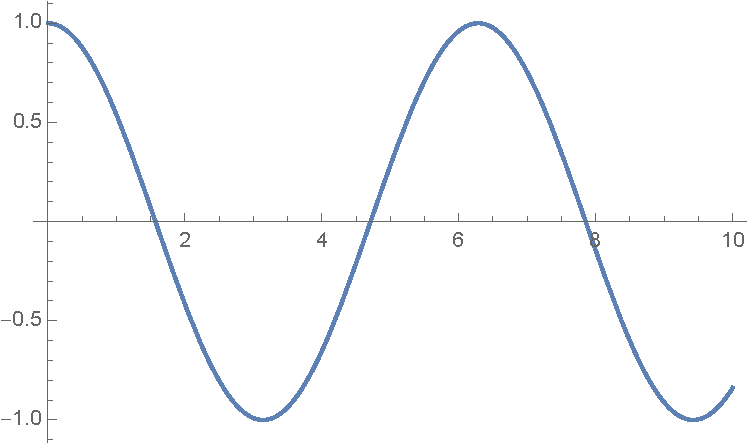
\includegraphics[width=6cm]{images/1_x.pdf}
\caption{(1) $(t, x(t))$}
\end{minipage}
%
\begin{minipage}{0.45\columnwidth}
\centering
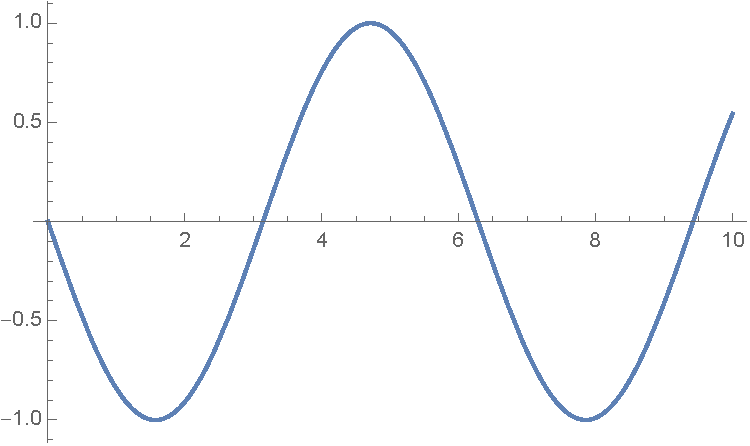
\includegraphics[width=6cm]{images/1_y.pdf}
\caption{(1) $(t, y(t))$}
\end{minipage}
\end{figure}

$N' = 200000$ とすると, \ $x^{(N')} = -8.3928e-01, \ \ y^{(N')} = 5.4416e-01$ である. \par
この値を, 真の解と見なす. 
\begin{table}[htbp]
\centering
\begin{tabular}{|c||c|c|c|c|} \hline
\textbf{$N$} & \textbf{$x^{(N)}$} & \textbf{$y^{(N)}$} & \textbf{$|x^{(N)}-x^{(N')}|$} & \textbf{$|y^{(N)}-y^{(N')}|$} \\ \hline
$100$ & $-1.4088e+00$ & $8.4851e-01$ & $5.6957e-01$ & $3.0435e-01$ \\ \hline
$200$ & $-1.0828e+00$ & $6.8933e-01$ & $2.4355e-01$ & $1.4518e-01$ \\ \hline
$300$ & $-9.9353e-01$ & $6.3895e-01$ & $1.5424e-01$ & $9.4796e-02$ \\ \hline
$400$ & $-9.5204e-01$ & $6.1445e-01$ & $1.1276e-01$ & $7.0294e-02$ \\ \hline
$500$ & $-9.2810e-01$ & $5.9999e-01$ & $8.8818e-02$ & $5.5831e-02$ \\ \hline
$600$ & $-9.1253e-01$ & $5.9045e-01$ & $7.3245e-02$ & $4.6290e-02$ \\ \hline
$700$ & $-9.0159e-01$ & $5.8368e-01$ & $6.2307e-02$ & $3.9527e-02$ \\ \hline
$800$ & $-8.9348e-01$ & $5.7864e-01$ & $5.4203e-02$ & $3.4482e-02$ \\ \hline
$900$ & $-8.8724e-01$ & $5.7473e-01$ & $4.7958e-02$ & $3.0576e-02$ \\ \hline
$1000$ & $-8.8228e-01$ & $5.7162e-01$ & $4.2999e-02$ & $2.7461e-02$ \\ \hline
\end{tabular}
\caption{(1) $|x^{(N)}-x^{(N')}|$と$|y^{(N)}-y^{(N')}|$}
\end{table}

表1より, 反復回数が増えるほど, 誤差の値は小さくなり, 解は真の解に近づいていることがわかる. \par
以下の図3は, $T = 10$ と固定した時の, $N = 100, 500, 1000, 10000, 100000$ における $(t, x(t))$, $(t, y(t))$, $(x(t)t, y(t))$ の振る舞いのグラフである. \\
($T = 10$ としたのは, $T = 100$ のグラフを出力したところ, グラフの振る舞いがわかりにくかった為である. )
\begin{figure}[htbp]
\centering
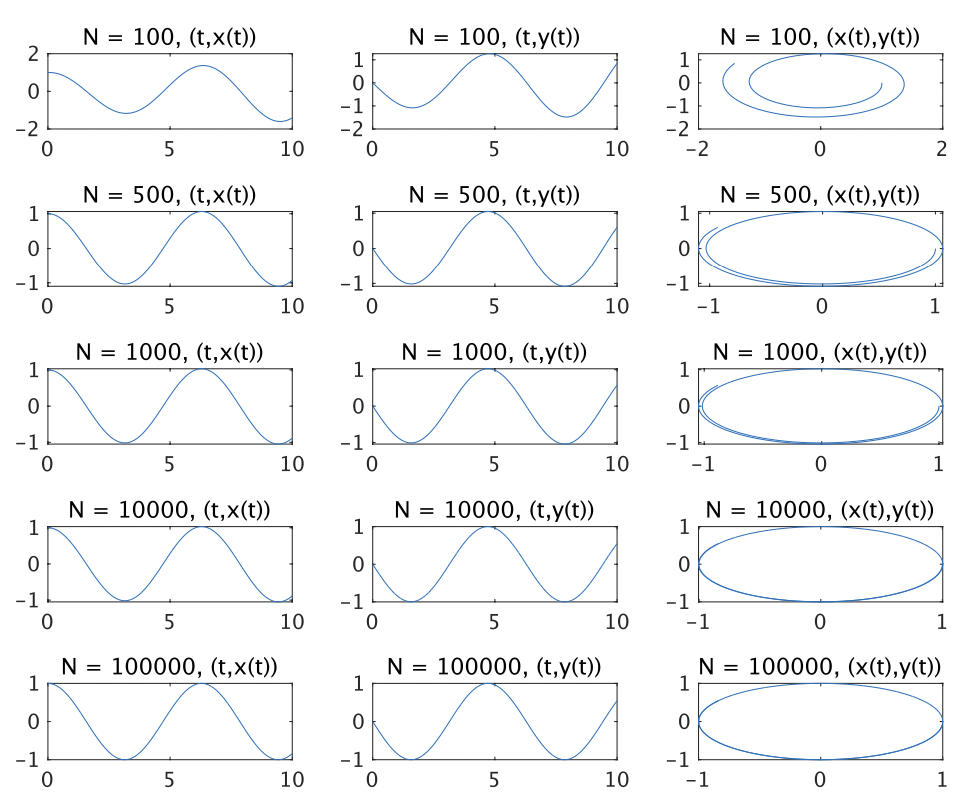
\includegraphics[width=15cm]{images/1_matlab.png}
\caption{(1) $(t, x(t))$, $(t, y(t))$, $(x(t)t, y(t))$ の振る舞い}
\end{figure}

\clearpage
%%%%%%%%%%%%%%%%%%%%%%%%%%%%%%%%%%%%%%%%%%%%%%%%%%%%%%%%%%%%%%%%%%%%%%%%%%%%%%%%%%%%%%%%%%%%%%%%%%%%%%%
\subsubsection{(2) $a_{11} = -1, \ a_{12} = 1, \ a_{21} = -4, \ a_{22} = 0$}
固有値:$\displaystyle \frac{-1+\sqrt{15}i}{2}, \frac{-1-\sqrt{15}i}{2}$. \ \ 対応する固有ベクトルは, $\begin{pmatrix} \frac{1-\sqrt{15}i}{8} \\ 1 \end{pmatrix}$, $\begin{pmatrix} \frac{1+\sqrt{15}i}{8} \\ 1 \end{pmatrix}$ である. \\
まず, (2)の場合の理論解は, 
\[\left\{ 
\begin{array}{l}
\displaystyle x(t) = e^{-\frac{1}{2}t}\left( \cos{\frac{\sqrt{15}}{2}t} - \frac{1}{\sqrt{15}}\sin{\frac{\sqrt{15}}{2}t}\right) \\ \\
\displaystyle y(t) = e^{-\frac{1}{2}t}\left(-\frac{8}{\sqrt{15}}\sin{\frac{\sqrt{15}}{2}t}\right) \ \ \ \ \ \ \ \ \ \ \ \ \ \ \ \ \ となる. \\
\end{array}
\right. \]
したがって, 理論解の $(t, x(t))$, $(t, y(t))$ の振る舞いは, 下の, 図4, 図5 のようになる. 

\begin{figure}[htbp]
\centering
\begin{minipage}{0.45\columnwidth}
\centering
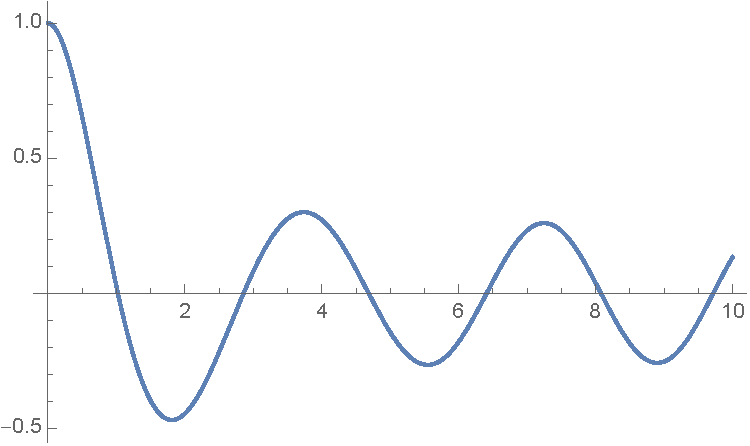
\includegraphics[width=6cm]{images/2_x.pdf}
\caption{(2) $(t, x(t))$}
\end{minipage}
%
\begin{minipage}{0.45\columnwidth}
\centering
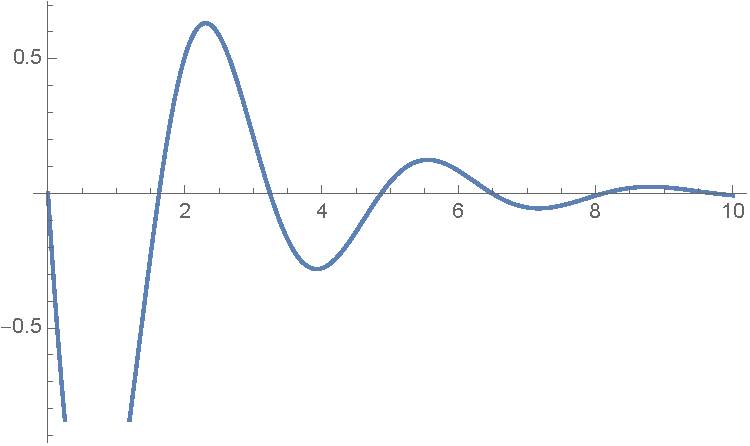
\includegraphics[width=6cm]{images/2_y.pdf}
\caption{(2) $(t, y(t))$}
\end{minipage}
\end{figure}

$N' = 200000$ とすると, \ $x^{(N')} = 5.0074e-03, \ \ y^{(N')} = -6.8713e-03$ である. \par
この値を, 真の解と見なす. 
\begin{table}[htbp]
\centering
\begin{tabular}{|c||c|c|c|c|} \hline
\textbf{$N$} & \textbf{$x^{(N)}$} & \textbf{$y^{(N)}$} & \textbf{$|x^{(N)}-x^{(N')}|$} & \textbf{$|y^{(N)}-y^{(N')}|$} \\ \hline
$100$ & $2.7626e-03$ & $-8.9122e-02$ & $2.2448e-03$ & $8.2251e-02$ \\ \hline
$200$ & $6.3189e-03$ & $-2.8284e-02$ & $1.3115e-03$ & $2.1413e-02$ \\ \hline
$300$ & $6.1271e-03$ & $-1.8514e-02$ & $1.1197e-03$ & $1.1643e-02$ \\ \hline
$400$ & $5.9116e-03$ & $-1.4775e-02$ & $9.0420e-04$ & $7.9033e-03$ \\ \hline
$500$ & $5.7557e-03$ & $-1.2830e-02$ & $7.4828e-04$ & $5.9588e-03$ \\ \hline
$600$ & $5.6429e-03$ & $-1.1645e-02$ & $6.3546e-04$ & $4.7739e-03$ \\ \hline
$700$ & $5.5586e-03$ & $-1.0850e-02$ & $5.5115e-04$ & $3.9785e-03$ \\ \hline
$800$ & $5.4935e-03$ & $-1.0280e-02$ & $4.8612e-04$ & $3.4084e-03$ \\ \hline
$900$ & $5.4420e-03$ & $-9.8514e-03$ & $4.3455e-04$ & $2.9801e-03$ \\ \hline
$1000$ & $5.4001e-03$ & $-9.5181e-03$ & $3.9273e-04$ & $2.6468e-03$ \\ \hline
\end{tabular}
\caption{(2) $|x^{(N)}-x^{(N')}|$と$|y^{(N)}-y^{(N')}|$}
\end{table}

表2より, $N = 100$ と $N = 200$ の間で大きく真の解に近づくことがわかる. \par
以下の図6は, $T = 10$ と固定した時の, $N = 100, 500, 1000, 10000, 100000$ における $(t, x(t))$, $(t, y(t))$, $(x(t)t, y(t))$ の振る舞いのグラフである. \\
($T = 10$ としたのは, $T = 100$ のグラフを出力したところ, グラフの振る舞いがわかりにくかった為である. )
\begin{figure}[htbp]
\centering
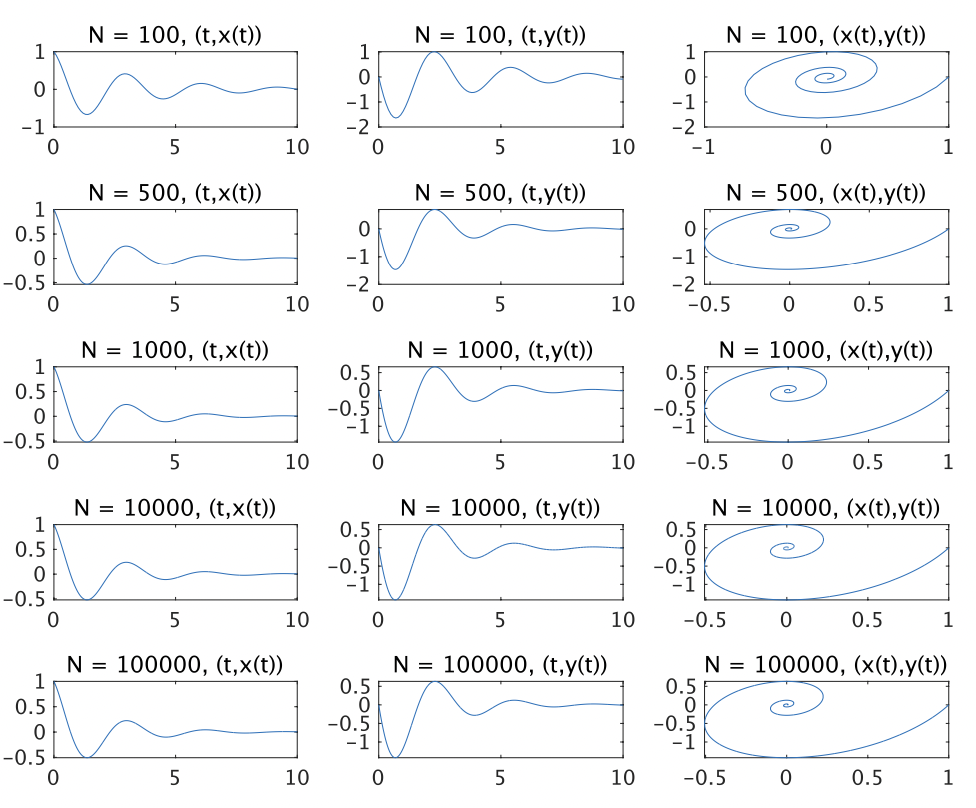
\includegraphics[width=15cm]{images/2_matlab.png}
\caption{(2) $(t, x(t))$, $(t, y(t))$, $(x(t)t, y(t))$ の振る舞い}
\end{figure}

\clearpage
%%%%%%%%%%%%%%%%%%%%%%%%%%%%%%%%%%%%%%%%%%%%%%%%%%%%%%%%%%%%%%%%%%%%%%%%%%%%%%%%%%%%%%%%%%%%%%%%%%%%%%%
\subsubsection{(3) $a_{11} = \ 1\ , \ a_{12} = 1, \ a_{21} = -4, \ a_{22} = 0$}
固有値:$\displaystyle \frac{1+\sqrt{15}i}{2}, \frac{1-\sqrt{15}i}{2}$. \ \ 対応する固有ベクトルは, $\begin{pmatrix} \frac{-\sqrt{15}i-1}{8} \\ 1 \end{pmatrix}$, $\begin{pmatrix} \frac{\sqrt{15}i-1}{8} \\ 1 \end{pmatrix}$ である. \\
まず, (3)の場合の理論解は, 
\[\left\{ 
\begin{array}{l}
\displaystyle x(t) = e^{\frac{1}{2}t}\left( \cos{\frac{\sqrt{15}}{2}t} + \frac{1}{\sqrt{15}}\sin{\frac{\sqrt{15}}{2}t}\right) \\ \\
\displaystyle y(t) = e^{\frac{1}{2}t}\left(-\frac{8}{\sqrt{15}}\sin{\frac{\sqrt{15}}{2}t}\right) \ \ \ \ \ \ \ \ \ \ \ \ \ \ \ \ \ となる. \\
\end{array}
\right. \]
したがって, 理論解の $(t, x(t))$, $(t, y(t))$ の振る舞いは, 下の, 図7, 図8 のようになる. 

\begin{figure}[htbp]
\centering
\begin{minipage}{0.45\columnwidth}
\centering
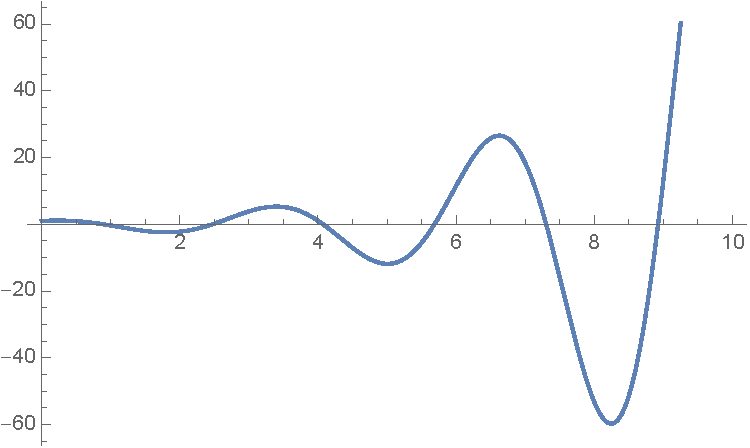
\includegraphics[width=6cm]{images/3_x.pdf}
\caption{(3) $(t, x(t))$}
\end{minipage}
%
\begin{minipage}{0.45\columnwidth}
\centering
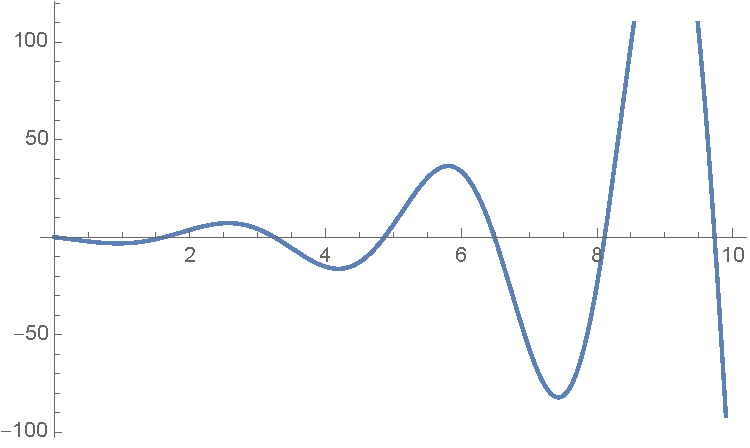
\includegraphics[width=6cm]{images/3_y.pdf}
\caption{(3) $(t, y(t))$}
\end{minipage}
\end{figure}

$N' = 200000$ とすると, \ $x^{(N')} = 1.4817e+02, \ \ y^{(N')} = -1.5109e+02$ である. \par
この値を, 真の解と見なす. 
\begin{table}[htbp]
\centering
\begin{tabular}{|c||c|c|c|c|} \hline
\textbf{$N$} & \textbf{$x^{(N)}$} & \textbf{$y^{(N)}$} & \textbf{$|x^{(N)}-x^{(N')}|$} & \textbf{$|y^{(N)}-y^{(N')}|$} \\ \hline
$100$ & $4.6943e+02$ & \ \ $8.3062e+02$ & $3.2126e+02$ & $9.8171e+02$ \\ \hline
$200$ & $3.3815e+02$ & \ \ $9.0057e+00$ & $1.8998e+02$ & $1.6010e+02$ \\ \hline
$300$ & $2.6808e+02$ & $-9.2259e+01$ & $1.1991e+02$ & $5.8832e+01$ \\ \hline
$400$ & $2.3462e+02$ & $-1.2142e+02$ & $8.6447e+01$ & $2.9669e+01$ \\ \hline
$500$ & $2.1548e+02$ & $-1.3346e+02$ & $6.7311e+01$ & $1.7630e+01$ \\ \hline
$600$ & $2.0319e+02$ & $-1.3952e+02$ & $5.5016e+01$ & $1.1574e+01$ \\ \hline
$700$ & $1.9465e+02$ & $-1.4297e+02$ & $4.6476e+01$ & $8.1231e+00$ \\ \hline
$800$ & $1.8838e+02$ & $-1.4511e+02$ & $4.0210e+01$ & $5.9797e+00$ \\ \hline
$900$ & $1.8359e+02$ & $-1.4653e+02$ & $3.5419e+01$ & $4.5620e+00$ \\ \hline
$1000$ & $1.7981e+02$ & $-1.4751e+02$ & $3.1641e+01$ & $3.5784e+00$ \\ \hline
\end{tabular}
\caption{(3) $|x^{(N)}-x^{(N')}|$と$|y^{(N)}-y^{(N')}|$}
\end{table}

表3より, 反復回数が増えるほど, 誤差の値は大きくなるとわかる. \par
以下の図9は, $T = 10$ と固定した時の, $N = 100, 500, 1000, 10000, 100000$ における $(t, x(t))$, $(t, y(t))$, $(x(t)t, y(t))$ の振る舞いのグラフである. \\
($T = 10$ としたのは, $T = 100$ のグラフを出力したところ, グラフの振る舞いがわかりにくかった為である. )
\begin{figure}[htbp]
\centering
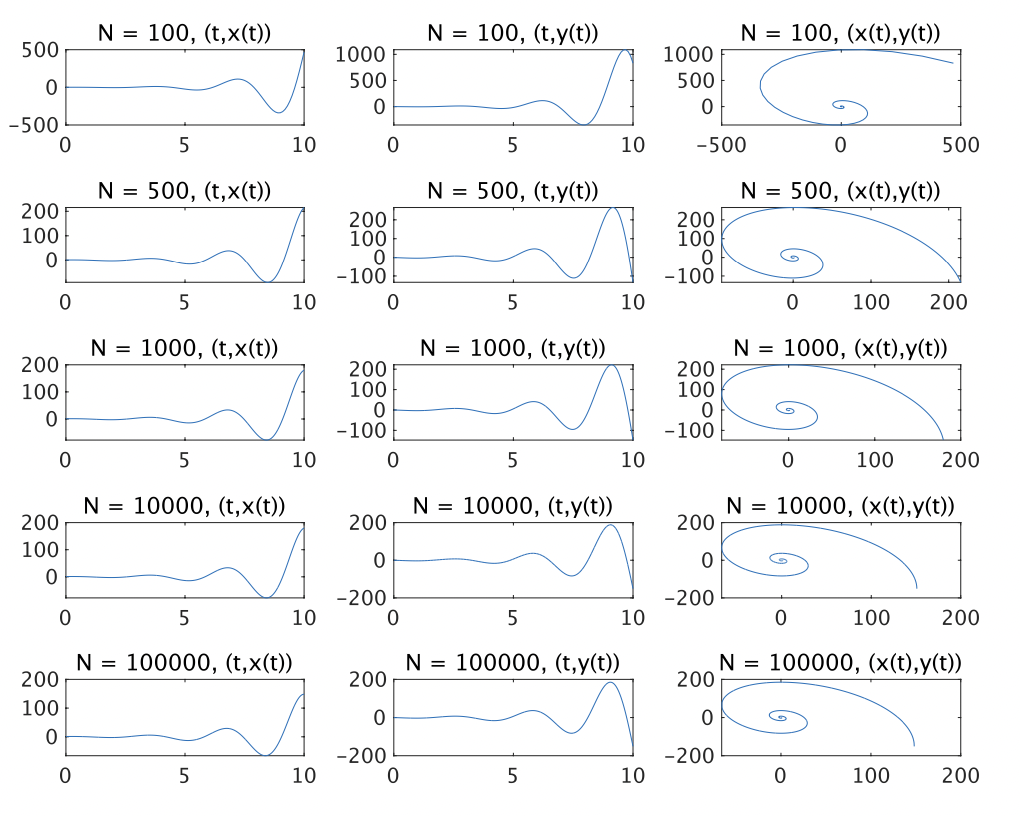
\includegraphics[width=15cm]{images/3_matlab.png}
\caption{(3) $(t, x(t))$, $(t, y(t))$, $(x(t)t, y(t))$ の振る舞い}
\end{figure}

\clearpage
%%%%%%%%%%%%%%%%%%%%%%%%%%%%%%%%%%%%%%%%%%%%%%%%%%%%%%%%%%%%%%%%%%%%%%%%%%%%%%%%%%%%%%%%%%%%%%%%%%%%%%%

%6.考察(理論的・数値的な側面からできる限り詳しく述べる)
\subsection{考察}
今回は, 解の動きをわかりやすくするため, 各パターンにおいて, $T = 10$ と固定した時の, $N = 100, 500, 1000, 10000, 100000$ における $(t, x(t))$, $(t, y(t))$, $(x(t)t, y(t))$ の振る舞いのグラフを出力した. \par
(1)の場合, $N$ を大きくすればするほど, $(x(t)t, y(t))$ の振る舞いのグラフは, 中心 $(0, 0)$, 半径 $1$ の円, つまり単位円に近づいているとわかる. つまり, 解の変化は一定(安定)していると考えられる. また, $(t, x(t))$, $(t, y(t))$ の振る舞いのグラフは, $N$ を大きくするほど, 理論解である三角関数の形に近似される. これにより, $N$ が大きくなるにつれて, 真の解との誤差は小くなり, 値は真の解へ近似されていることがわかる. \par
(2)の場合, $(x(t)t, y(t))$ の振る舞いのグラフは, 点 $(1, 0)$ から, 点 $(0, 0)$  へ徐々に近づいていることがわかる. つまり, 解の変化は一定(安定)していると考えられる. また, $(t, x(t))$, $(t, y(t))$ の振る舞いのグラフは, ともに $0$ に収束するグラフとなっている. 理論解で, $e^{-\frac{1}{2}t}$が式にかけられている点から徐々に $0$ に収束すると予想されたが, $N$ を大きくし, 実際に実験することによって明らかになった. \par
(3)の場合, $(x(t)t, y(t))$ の振る舞いのグラフは, (2)と逆になっているように見える. これは, (2)では $a_{11} = -1$ , (3)では $a_{11} = 1$ と $a_{11}$ の符号が異なったからではないかと考えた. しかし, よく見ると, (2)は一定の値(点 $(0, 0)$ )へ近づいているが, (3) では一定の値に近づていることが読み取りにくい. また, $N$ を増やすほど, 誤差の値が大きくなっている. つまり, (1) (2) とは違い, 解が一定(安定)しているとは言えない. 反復回数を増やせば増やすほど, 誤差が大きくなる点については, 直感と異なる結果となった. 今後のさらなる実験や学修を伴う課題としたい. 


%7.結論(分かった事実や残された課題,新たに見つかった問題点など)
\subsection{結論}
連立線形常微分方程式の解の安定性は, 行列Aの固有値によって決まる. 固有値の実部がすべて非正ならば「リアプノフ安定」, 固有値の実部がすべて負ならば 「漸近安定」, ある固有値の実部が正ならば 「不安定」となる. 
まず, 「リアプノフ安定」とは, すべての解が平衡解の付近に止まり続ける安定性である. 次に, 「漸近安定」とは, すべての解が平衡解へ向かう安定性である. 最後に, 「不安定」とは, ある解が平衡解の付近から遠ざかっていくため, 安定性を持たないという状況である. \par
今回扱った3つの連立線形常微分方程式をこれに当てはめて考えてみる. (1)は, 固有値 $i, -i$ , 実部はともに $0$ であるため, リアプノフ安定である. $(x(t)t, y(t))$ の振る舞いのグラフが単位円に近づいていることからもわかる. (2)は, 固有値 $\frac{-1+\sqrt{15}i}{2}, \frac{-1-\sqrt{15}i}{2}$ , 実部はともに, $-\frac{1}{2}$ であるため, 漸近安定である. $(x(t)t, y(t))$ の振る舞いのグラフが点 $(0, 0)$ に近づいていることからもわかる. (3)は, 固有値 $\frac{1+\sqrt{15}i}{2}, \frac{1-\sqrt{15}i}{2}$ , 実部はともに $\frac{1}{2}$ であるため, 不安定である. $(x(t)t, y(t))$ の振る舞いのグラフが安定していないということがいえた. 



\clearpage
%%%%%%%%%%%%%%%%%%%%%%%%%%%%%%%%%%%%%%%%%%%%%%%%%%%%%%%%%%%%%%%%%%%%%%%%%%%%%%%%%%%%%%%%%%%%%%%%%%%%%%%%%%%%%%%%%%%%%%%%%%%%%%%%%%%%%%%%%%%%%%%%%%%%%%%%%%%%%%%%%%%%%%%%%%%%%%%%%%%%%%%%%%%%%%%%%%%%%%%%%%%%%%
\section{(d)(拡散項なしの)藤田方程式}
%3.問題設定(扱う方程式や解法,パラメータの設定など)
\subsection{問題設定}
\[\left\{ 
\begin{array}{l}
\displaystyle \frac{du}{dt} = |u|^{p-1}u\ \ \ \ 0 < t < T, \\ \\
u(0) = u_{0} > 0
\end{array}
\right.\]
\\
ここで, 実数 $p$ はパラメータである. \\
様々な $p$ に対して(例えば, $p \leq 0$, $0 < p \leq 1$, $p > 1$ )解の挙動を調べよ. \\
注意 : $p > 1$ のとき, 解がある時間 $T_{0}$ で爆発する($ \lim_{t \to T_{0}}u(t) \rightarrow \infty$ )ので, 適当な $T$ で計算を止めなければならない. ただし, $T$ が小さすぎると, 爆発の様子が見えない. 

% 4.理論(分かっている理論的な事実や解析結果,また自身の予想など)
\subsection{理論}
$\displaystyle \frac{du}{dt} = \Delta u + f(u)$ は, 反応拡散方程式である. この式において、 $u(x, t)$ は温度(または物質の濃度)で, $\Delta u$ は拡散項, $f(u)$ は反応項と呼ばれる. ( $f(u) = 0$ のときは, 熱や粒子の拡散を表す熱方程式(拡散方程式)であるが, 反応方程式では $0$ でない場合を考える. )この方程式が数学的に扱うことが難しくなるため, 派生させた方程式を, 非線形熱方程式という. $\displaystyle \frac{du}{dt} = \Delta u + u^{p}$ と表される. この方程式を先駆的に研究した数学者・藤田宏さんの名前をとり, 藤田方程式と呼ばれる. \par
今回は, 拡散項なしの藤田方程式を扱うため, 方程式の形は $\displaystyle \frac{du}{dt} = |u|^{p-1}u$ となっている. 
\begin{enumerate}
\renewcommand{\theenumi}{\roman{enumi}}
\renewcommand{\labelenumi}{\theenumi)}
\renewcommand{\labelenumii}{\alph{enumii})}
\item $u < 0$ のとき, \\
$\displaystyle \frac{du}{dt} = -u^{p}$ \ \ $\Leftrightarrow$ \ \ $u^{-p} du = -dt$ \\
\begin{enumerate}
\item $p \neq 1$ のとき, \\
$\displaystyle \frac{1}{1-p}u^{1-p} = -t + C_{1}$ \ \ $\Leftrightarrow$ \ \ $u^{1-p} = (p-1)t + C_{2}$ \\
よって, $\displaystyle u(t) = (p-1)t^{\frac{1}{1-p}} + C_{3}$ \\
また, $u(0) = C_{3} = u_{0} > 0$ より, $0 < C_{3}$ \\
\item $p = 1$ のとき, \\
$\displaystyle \frac{1}{u}du = -dt$ \ \ $\Leftrightarrow$  \ \ $\log{|u|} = -t + C_{4}$ \\
よって, $\displaystyle u(t) = C_{5}e^{t}$ \\
また, $u(0) = C_{5} = u_{0} > 0$ より, $0 < C_{5}$ \\
\end{enumerate}
\rightline{( $C_{1}, C_{2}, C_{3}, C_{4}, C_{5}$ は任意定数)}

\item $u = 0$ のとき, \\
$\displaystyle \frac{du}{dt} = 0$ \ \ $\Leftrightarrow$ \ \ $u(t) = C_{6}$ \\
また, $u(0) = C_{6} = u_{0} > 0$ より, $0 < C_{6}$ \\
\rightline{( $C_{6}$ は任意定数)}

\item $u > 0 $ のとき, \\
$\displaystyle \frac{du}{dt} = u^{p}$ \ \ $\Leftrightarrow$ \ \ $u^{-p} du = dt$ \\
\begin{enumerate}
\item $p \neq 1$ のとき, \\
$\displaystyle \frac{1}{1-p}u^{1-p} = t + C_{7}$ \ \ $\Leftrightarrow$ \ \ $u^{1-p} = (1-p)t + C_{8}$ \\
よって, $\displaystyle u(t) = (1-p)t^{\frac{1}{1-p}} + C_{9}$ \\
また, $u(0) = C_{9} = u_{0} > 0$ より, $0 < C_{9}$ \\
\item $p = 1$ のとき, \\
$\displaystyle \frac{1}{u}du = dt$ \ \ $\Leftrightarrow$  \ \ $\log{|u|} = t + C_{10}$ \\
よって, $\displaystyle u(t) = C_{11}e^{t}$ \\
また, $u(0) = C_{11} = u_{0} > 0$ より, $0 < C_{11}$ \\
\rightline{( $C_{7}, C_{8}, C_{9}, C_{10}, C_{11}$ は任意定数)}
\end{enumerate}

\end{enumerate}


%\displaystyle \frac{du}{dt}

%5.実験結果(表やグラフなどを利用して見やすくする)
\subsection{実験結果}
$N = 10$ で固定し, $T$ と $p$ を変化させたときの変化を調べた.\par
$p\leq 0$ として $p = -5$ を, $0<p\leq1$ として $p = 0.5$ を, $p>1$ として $p = 5$ を使用した. 
\begin{table}[htbp]
\centering
\begin{tabular}{|c||c|c|c|} \hline
\textbf{$T$} & \textbf{$p = -5$} & \textbf{$p = 0.5$} & \textbf{$p = 5$} \\ \hline\hline
$100$ & $1.1001e+01$ & $1.7697e+03$ & \ \ \ \ \ \ Inf\ \ \ \ \ \ \ \\ \hline
$500$ & $5.1000e+01$ & $3.7023e+04$ & Inf \\ \hline
$1000$ & $1.0100e+02$ & $1.3972e+05$ & Inf \\ \hline
$10000$ & $1.0010e+03$ & $1.2002e+07$ & Inf \\ \hline
$100000$ & $1.0001e+04$ & $1.0701e+09$ & Inf \\ \hline
\end{tabular}
\caption{(拡散項なしの)藤田方程式}
\end{table}
\clearpage

\begin{figure}[htbp]
\centering
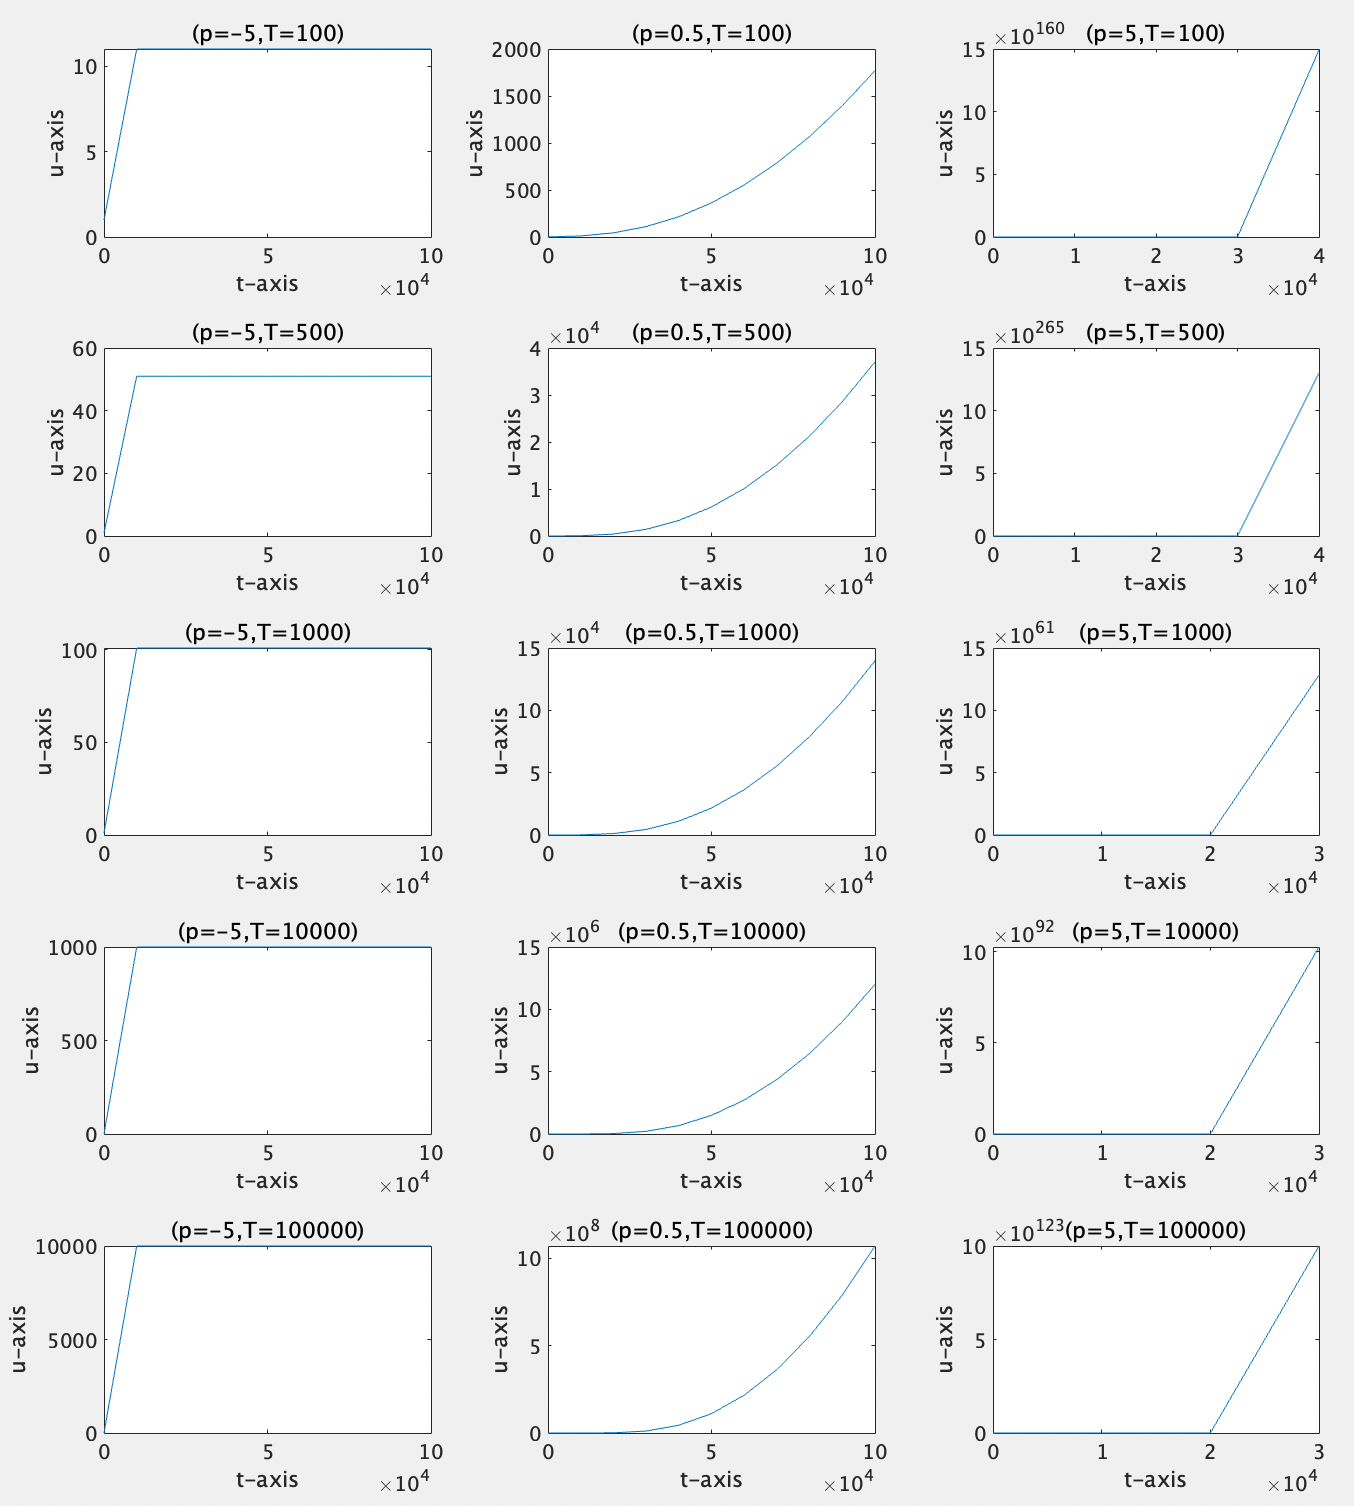
\includegraphics[width=15cm]{images/d_matlab.png}
\caption{(拡散項なしの)藤田方程式 (N = 10 , T と p を変化させた)}
\end{figure}

\clearpage
%6.考察(理論的・数値的な側面からできる限り詳しく述べる)
\subsection{考察}
$N = 10$ で固定し, $T = 100, 500, 1000, 10000, 100000$ , $p = -5, \ 0.5, \ 5$ と変化させ実験をおこなった.\par
$p = -5$ ( $p\leq 0$ )のとき, 解は $t = 0$ から $t = 2.5$ のあたりで急速に大きくなり, その後は一定のまま変動がない. $T$ の値を大きくすればするほど, 一定になったときの値が大きくなるとわかる. また, この値はおよそ $\frac{T}{10}$ になっていると読み取れる. \par
$p = 0.5$ ( $0<p\leq1$ )のとき, 解は指数関数的に増加している. \par
$p = 5$ ( $p>1$ )のとき, 解は $T = 2$ から先で急速に大きくなる. これは, 課題の注意にあった「$p > 1$ のとき, 解がある時間 $T_{0}$ で爆発する($ \lim_{t \to T_{0}}u(t) \rightarrow \infty$ )」の話であると考えた. $T_{0} = 2$ であると推測できる. 

%7.結論(分かった事実や残された課題,新たに見つかった問題点など)
\subsection{結論}
課題の注意にあるように, $p > 1$ のとき, 解がある時間 $T_{0}$ で爆発する($ \lim_{t \to T_{0}}u(t) \rightarrow \infty$ ). このような現象を, 解の爆発(blow-up)といい, このときの解を, 「爆発解」その時間 $T_{0}$ を爆発時間と呼ぶ. 反対に, 爆発せず存在し続ける解は「時間大域解」と呼ばれている. \\
$p_{F} = \frac{N + 2}{N}$ とすると, 正値解(最大値原理より, 解が $t > 0$ において正になることが保証される)は, 
\begin{itemize}
\item[(1)] $ < p < p_{F}$ ならば, すべての解は有限時間で爆発し, 解は爆発解となる. 
\item[(2)] $p_{F} < p$ ならば, 時間大域解が存在する. 
\end{itemize}
という結果になる. ( $p_{F}$ は藤田指数と呼ばれる. )\\
よって, 今回の実験において, $p = 0.5,\ 5$ の場合はこれに当てはまるとわかる. \\
また, $p = -5$, つまり $t \leqq 0$ の場合については, 今後の課題としたい. \\
\clearpage
%%%%%%%%%%%%%%%%%%%%%%%%%%%%%%%%%%%%%%%%%%%%%%%%%%%%%%%%%%%%%%%%%%%%%%%%%%%%%%%%%%%%%%%%%%%%%%%%%%%%%%%%%%%%%%%%%%%%%%%%%%%%%%%%%%%%%%%%%%%%%%%%%%%%%%%%%%%%%%%%%%%%%%%%%%%%%%%%%%%%%%%%%%%%%%%%%%%%%%%%%%%%%%
%8.感想
\section{感想}
今回のレポートでは, 結果から何かを十分に考察するだけの知識が自分に不足しているように感じた. その一方で, すでに学習していた微分方程式の知識が役に立つことが多くあり, 学修すること・ひとつの物事に対して多面的な思考で考えることの重要性や学びの深さを感じた. プログラムをして具体的に値を代入して求める解のグラフが, 理論的に式変形をして求めた理論解のグラフに近づいていた点, とても面白さを感じた. \par
常微分方程式をもっと深く理解するには, 身近な現象に触れ, 数式で表したときの解の挙動などを調べるなど, 一層自主的な学修活動が必要であると実感した. \par
MATLABを用いて解の振る舞いのグラフを出力したが, MATLABはわからないことが多かったため, MathWorks ヘルプセンターを参照しながらコードを書いた. 「tiledlayout(5,3) \ nexttile」といった, グラフを一覧で出力する方法など, この課題がなければ知らなかったであろうことを知ることができ, 積極的に利用できたため, MATLABに対する理解度があがったと感じた. \par



\clearpage

%%%%%
\section{使用したソースコード}
使用したソースコードの一部を以下に記載する. 
\begin{lstlisting}[caption={表3 \ $N = 100$ の場合},style=MATLABStyle]
A = [1,1;-4,0]
a11 = 1;
a12 = 1;
a21 = -4;
a22 = 0;

a = 0;
b = 10;

n100 = 100;
h = (b-a)/n100;
t100 = a:h:b;

y = zeros(size(t100));
x = zeros(size(t100));

x100=zeros(size(t100));
y100=zeros(size(t100));

x(1) = 1;
y(1) = 0;

x100(1) = 1;
y100(1) = 0;

for i=1: length(t100)-1
    x(i+1) = x(i)+h*(a11*x(i)+a12*(y(i)));
    y(i+1) = y(i)+h*(a21*x(i)+a22*(y(i)));
    x100(i+1)=x(i+1);
    y100(i+1)=y(i+1);
end

disp('----');
format shortE
disp('x^(100)');
disp(x100(n100+1));
disp('y^(100)');
disp(y100(n100+1));
disp('x^(100)-x^(n)');
disp(abs(x100(n100+1)-x200000(n200000+1)));
disp('y^(100)-y^(n)');
disp(abs(y100(n100+1)-y200000(n200000+1)));
\end{lstlisting}

\begin{lstlisting}[caption={図10 (拡散項なしの)藤田方程式 (N = 10 , T と p を変化させた)},style=MATLABStyle]
n = 10;
a = 0;

%%%%%%%%%%%%%%%%%%%%%%%%%%%%%%%%%%%%%%%%%
%y1100→p=1,T=100
%y2500→p=2,T=500
%y31000→p=3,T=1000  の意味
%%%%%%%%%%%%%%%%%%%%%%%%%%%%%%%%%%%%%%%%%

% T = 100 %%%%%%%%%%%%%%%%%%%%%%%%%%%%%%%
b = 100;

h = (b-a)/n;
t = a:h:b;

p = -5;
y1100 = zeros(size(t));
y1100(1) = abs(1);

for i = 1:length(t)-1
    y1100(i+1)=y1100(i)+h*((abs(y1100(i))^(p-1))*y1100(i));
end

format shortE
disp(y1100(n+1));

p2 = 0.5;
y2100 = zeros(size(t));
y2100(1)=y1100(1);

for i=1:length(t)-1
    y2100(i+1)=y2100(i)+h*(y2100(i)^(p2-1)*y2100(i));
end

format shortE
disp(y2100(n+1));

p3 = 5;
y3100 = zeros(size(t));
y3100(1)=y1100(1);

for i=1:length(t)-1
    y3100(i+1)=y3100(i)+h*(y3100(i)^(p3-1)*y3100(i));
end

format shortE
disp(y3100(n+1));


% T = 500 %%%%%%%%%%%%%%%%%%%%%%%%%%%%%%%
b = 500;
h = (b-a)/n;
t = a:h:b;

p = -5;
y1500 = zeros(size(t));
y1500(1) = abs(1);

for i = 1:length(t)-1
    y1500(i+1)=y1500(i)+h*((abs(y1500(i))^(p-1))*y1500(i));
end

format shortE
disp(y1500(n+1));

p2 = 0.5;
y2500 = zeros(size(t));
y2500(1)=y1500(1);

for i=1:length(t)-1
    y2500(i+1)=y2500(i)+h*(y2500(i)^(p2-1)*y2500(i));
end

format shortE
disp(y2500(n+1));

p3 = 5;
y3500 = zeros(size(t));
y3500(1)=y1500(1);

for i=1:length(t)-1
    y3500(i+1)=y3500(i)+h*(y3500(i)^(p3-1)*y3500(i));
end

format shortE
disp(y3500(n+1));

% T = 1000 %%%%%%%%%%%%%%%%%%%%%%%%%%%%%%%
b = 1000;
h = (b-a)/n;
t = a:h:b;

p = -5;
y11000 = zeros(size(t));
y11000(1) = abs(1);

for i = 1:length(t)-1
    y11000(i+1)=y11000(i)+h*((abs(y11000(i))^(p-1))*y11000(i));
end

format shortE
disp(y11000(n+1));

p2 = 0.5;
y21000 = zeros(size(t));
y21000(1)=y11000(1);

for i=1:length(t)-1
    y21000(i+1)=y21000(i)+h*(y21000(i)^(p2-1)*y21000(i));
end

format shortE
disp(y21000(n+1));

p3 = 5;
y31000 = zeros(size(t));
y31000(1)=y11000(1);

for i=1:length(t)-1
    y31000(i+1)=y31000(i)+h*(y31000(i)^(p3-1)*y31000(i));
end

format shortE
disp(y31000(n+1));

% T = 10000 %%%%%%%%%%%%%%%%%%%%%%%%%%%%%%%
b = 10000;
h = (b-a)/n;
t = a:h:b;

p = -5;
y110000 = zeros(size(t));
y110000(1) = abs(1);

for i = 1:length(t)-1
    y110000(i+1)=y110000(i)+h*((abs(y110000(i))^(p-1))*y110000(i));
end

format shortE
disp(y110000(n+1));

p2 = 0.5;
y210000 = zeros(size(t));
y210000(1)=y110000(1);

for i=1:length(t)-1
    y210000(i+1)=y210000(i)+h*(y210000(i)^(p2-1)*y210000(i));
end

format shortE
disp(y210000(n+1));

p3 = 5;
y310000 = zeros(size(t));
y310000(1)=y110000(1);

for i=1:length(t)-1
    y310000(i+1)=y310000(i)+h*(y310000(i)^(p3-1)*y310000(i));
end

format shortE
disp(y310000(n+1));

% T = 100000 %%%%%%%%%%%%%%%%%%%%%%%%%%%%%%%
b = 100000;
h = (b-a)/n;
t = a:h:b;

p = -5;
y1100000 = zeros(size(t));
y1100000(1) = abs(1);

for i = 1:length(t)-1
    y1100000(i+1)=y1100000(i)+h*((abs(y1100000(i))^(p-1))*y1100000(i));
end

format shortE
disp(y1100000(n+1));

p2 = 0.5;
y2100000 = zeros(size(t));
y2100000(1)=y1100000(1);

for i=1:length(t)-1
    y2100000(i+1)=y2100000(i)+h*(y2100000(i)^(p2-1)*y2100000(i));
end

format shortE
disp(y2100000(n+1));

p3 = 5;
y3100000 = zeros(size(t));
y3100000(1)=y1100000(1);

for i=1:length(t)-1
    y3100000(i+1)=y3100000(i)+h*(y3100000(i)^(p3-1)*y3100000(i));
end

format shortE
disp(y3100000(n+1));

%%%%%%%%%%%%%%%%%%%%%%%%%%%%%%%%

tiledlayout(5,3)

% N = 100 %%%%%%%%%

nexttile
plot(t,y1100,'-')
title('(p=-5,T=100)')
xlabel('t-axis')
ylabel('u-axis')

nexttile
plot(t,y2100,'-')
title('(p=0.5,T=100)')
xlabel('t-axis')
ylabel('u-axis')

nexttile
plot(t,y3100,'-')
title('(p=5,T=100)')
xlabel('t-axis')
ylabel('u-axis')

% N = 500 %%%%%%%%%

nexttile
plot(t,y1500,'-')
title('(p=-5,T=500)')
xlabel('t-axis')
ylabel('u-axis')

nexttile
plot(t,y2500,'-')
title('(p=0.5,T=500)')
xlabel('t-axis')
ylabel('u-axis')

nexttile
plot(t,y3500,'-')
title('(p=5,T=500)')
xlabel('t-axis')
ylabel('u-axis')

% N = 1000 %%%%%%%%%

nexttile
plot(t,y11000,'-')
title('(p=-5,T=1000)')
xlabel('t-axis')
ylabel('u-axis')

nexttile
plot(t,y21000,'-')
title('(p=0.5,T=1000)')
xlabel('t-axis')
ylabel('u-axis')

nexttile
plot(t,y31000,'-')
title('(p=5,T=1000)')
xlabel('t-axis')
ylabel('u-axis')

% N = 10000 %%%%%%%%%

nexttile
plot(t,y110000,'-')
title('(p=-5,T=10000)')
xlabel('t-axis')
ylabel('u-axis')

nexttile
plot(t,y210000,'-')
title('(p=0.5,T=10000)')
xlabel('t-axis')
ylabel('u-axis')

nexttile
plot(t,y310000,'-')
title('(p=5,T=10000)')
xlabel('t-axis')
ylabel('u-axis')

% N = 100000 %%%%%%%%%

nexttile
plot(t,y1100000,'-')
title('(p=-5,T=100000)')
xlabel('t-axis')
ylabel('u-axis')

nexttile
plot(t,y2100000,'-')
title('(p=0.5,T=100000)')
xlabel('t-axis')
ylabel('u-axis')

nexttile
plot(t,y3100000,'-')
title('(p=5,T=100000)')
xlabel('t-axis')
ylabel('u-axis')

\end{lstlisting}

\clearpage
%%%%%%%%%%%%%%%%%%%%%%%%%%%%%%%%%%%%%%%%%%%%%%%%%%%%%%%%%%%%%%%%%%
%9.参考文献(参考書や Web サイトなどを参考にした場合は必ず明記する) 文献の場合は,著者,タイトル,出版社,出版年度を書き,HP の場合は,著者,タイト ル,URL,最終更新(もしくは確認)日時を書くこと
\phantomsection % しおりの位置を調整
\addcontentsline{toc}{section}{参考文献} % 参考文献を目次に載せる
\begin{thebibliography}{99}
\bibitem{okamrura17} 所属大学の授業資料 \\
\bibitem{okamrura17} 古屋茂. 新版 微分方程式入門. サイエンス社, 2022. \\
\bibitem{okamura17} 奥村晴彦 / 黒木裕介. \LaTeX2$\varepsilon$ 美文書作成入門. 技術評論社, 2020\\
\bibitem{okamura17} MathWorks ヘルプセンター (閲覧日:2022.8.1)\\
 \url{https://jp.mathworks.com/help/matlab/index.html?s_tid=CRUX_lftnav}.\\
\bibitem{okamura17} 木村すらいむ. 趣味の大学数学 読み物としての数学入門サイト(閲覧日:2022.8.2)\\
 \url{https://math-fun.net/20180720/789/}.\\
 \url{https://math-fun.net/20190725/2377/#i}
\end{thebibliography}
\end{document}
